%%\documentclass{article}
\documentclass[12pt,twoside,a4paper]{scrbook}

\usepackage{geometry}
%\usepackage{amsmath, amssymb, amsthm}
\usepackage{graphicx}
\usepackage{color}
%\usepackage{ifthen}
%\usepackage{wrapfig}
%\usepackage{framed}
\usepackage{framed}
%\usepackage{enumitem}
\usepackage{listings} 
\usepackage{hyperref}
%\usepackage[numbers,sort&compress]{natbib} 


\geometry{left=3.5cm,textwidth=15cm,top=3cm,textheight=23cm}


\newenvironment{history}
{
 \begin{framed}
  \begin{minipage}{0.9\textwidth}
   { \footnotesize
    Historic remark:
   }
}
{
  \end{minipage}
 \end{framed}  
}


\lstdefinelanguage{cCCode}[]{C}{
  basicstyle=\small,
  stringstyle=\color{red},
  keywordstyle=\color{blue},
  commentstyle=\color{grey}\slshape,
  morekeywords={linestyle,linetype,linewidth,linecolor,pointtype,nohidden3d,hidden3d,palette,lt,lw,lc,pt,ps,fd,fill,fs,ls},
  framexleftmargin=1mm, framextopmargin=1mm, frame=shadowbox,
  rulesepcolor=\color{grey}
}
    
    
\lstnewenvironment{code}[1][]{
\lstset{
 language=cCCode,#1
}}{}
    
    

%
% Miriam hat 16 Seiten und dann pro Paper eine Seite Vorwort
% Michael hat 30 Seiten inkl einer Section pro Paper
%
%

%\newenvironment{history}
{
 \begin{framed}
  \begin{minipage}{0.9\textwidth}
   { \footnotesize
    Historic remark:
   }
}
{
  \end{minipage}
 \end{framed}  
}


\lstdefinelanguage{cCCode}[]{C}{
  basicstyle=\small,
  stringstyle=\color{red},
  keywordstyle=\color{blue},
  commentstyle=\color{grey}\slshape,
  morekeywords={linestyle,linetype,linewidth,linecolor,pointtype,nohidden3d,hidden3d,palette,lt,lw,lc,pt,ps,fd,fill,fs,ls},
  framexleftmargin=1mm, framextopmargin=1mm, frame=shadowbox,
  rulesepcolor=\color{grey}
}
    
    
\lstnewenvironment{code}[1][]{
\lstset{
 language=cCCode,#1
}}{}
    
    

\begin{document}

 
\begin{titlepage}

{ \large
  \begin{center}

  TECHNISCHE UNIVERSIT\"AT M\"UNCHEN \\
%  Technische Universit\"at M\"unchen\\
  \vspace{.3cm} 
  Department of Informatics \\
  Scientific Computing

  \vspace{4cm}
   Habilitationsverfahren Dr.~rer.~nat.~Tobias Weinzierl
  
  \vspace{1.5cm}

{\Huge
Cumulative Habilitation
}
\\
\vspace{1cm}
and 
\\
\vspace{0.6cm}
{\Huge
Progress Report\\
}

%   Dr.~rer.~nat.~Tobias Weinzierl
  \vspace{1.5cm}

%  \today
  \end{center}
}


\end{titlepage}


 \thispagestyle{empty}
 \newpage
 \cleardoublepage 

 \pagestyle{plain}
 \pagenumbering{roman}
 \chapter{Preamble}


\Peano\ is an open source framework for solvers on dynamically adaptive
Cartesian meshes.
Its core is built with C++, but many tools around it are written in Python.
\Peano\  is based upon the fact that spacetrees, a generalisation of the classical octree concept, yield a cascade of adaptive Cartesian grids. Consequently, any spacetree traversal is equivalent to an element-wise traversal of the hierarchy of the adaptive Cartesian grids. The software \Peano\  realises such a grid traversal and storage algorithm, and it provides hook-in points for applications performing per-element, per-vertex, and so forth operations on the grid. It also provides interfaces for dynamic load balancing, sophisticated geometry representations, and other features. Some properties are enlisted below.

Peano is currently available in its fourth generation. 
The development of the original set of Peano codes started around 2002.
2005-2009, we merged these codes into one Peano kernel (2nd generation). 
In 2009, I started a complete reimplementation of the kernel with special
emphasis on reusability, application-independent design and the support for rapid prototyping. 
This third generation of the code ended around 2019 when we released the
ExaHyPE code---a hyperbolic equation system solver engine which uses Peano's
AMR meshes.
The current guidebook discusses \Peano\ , which reuses ideas and lessons learned
from Peano~3 as well as lots of code buildling blocks, but can be seen as a
major rewrite starting from scratch.



\Peano\ has been the code base for multiple projects over the past years.
The most prominent one is likely ExaHyPE.
The first generation of ExaHyPE has been a stand-alone projects using Peano
as one required library or framework out of many.
The second generation, \ExaHyPE, is merged into \Peano as spin-off.
This document therefore covers \ExaHyPE, too.




\section*{Dependencies and prerequisites}

\Peano's core is plain C++17 code. 
We however use a whole set of tools around it:

\begin{itemize}
  \item GNU autotools (automake) to set up the system (required).
  \item C++17-compatible C++ compiler (required).
  \item Python3 (optional; not required if you work only with the C++
  baseline).
  \item MPI2 (optional). MPI's multithreaded support is required.
  \item Intel's Threading Building Blocks or OpenMP 5. We also can work with C++
  threads, but found their performance suboptimal.
  \item The Visualization Toolkit (VTK) if you want to use the built-in
  visualisation facilities (optional).
  \item Doxygen if you want to create HTML pages of PDFs of the in-code
  documentation.
\end{itemize}

\begin{remark}
I test and maintain \Peano\  for Linux only.
If you prefer Windows or MacOS, it should work as long as you provide the
mandatory tools from above, but I won't be able to help.
\end{remark}


\begin{center}
 \begin{tabular}{|l|l|p{8cm}|}
  \hline
   Software & Version & Remarks \\
  \hline
   GNU g++ & 7.5 or older & Works with \Peano\ core but not with some extensions
   such as \ExaHyPE. \\
   GNU g++ & 9.3.1 & Current development version. Works. \\
  \hline
   Intel icpc & 19.1 & Works with \Peano\ and all
   extensions such as \ExaHyPE. Tests with Intel Fortran have been successful,
   too. \\
  \hline
   VTK & 7--9 & Supported by \Peano. Default is 8, i.e.~if you need other
   version, you have to inform configure (see Chapter \ref{chapter:postprocessing}). \\
   \hline
   Python & 3 & Development version. Python 2 is not supported by frontend. \\
   \hline
 \end{tabular}
\end{center}

\section*{Who should read this document}

This cookbook is written similar to a tutorial in a hands-on style.
Therefore, it also contains lots of source code snippets.
If you read through a chapter, you should immediately be able to re-program the
presented details in your code and use the ideas.

Therefore, this cookbook is written for people that have a decent programming
background as well as scientific computing knowledge.
% Some background in the particular application area's algorithms for some
% chapters also is required. 
It is a cookbook that shall help readers to translate their scientific vision
into a working code quickly.


\section*{How the text is organised}

% This book covers a variety of problems I have tackled with Peano when I wrote
% scientific papers.
% There is no overall read thread through the document.
% I recommend to start reading some chapters and then jump into chapters
% that are of particular interest.
% Whenever something comes to my mind that should be added, I will add it.
If you feel something is urgently missing and deserves a chapter or things
remain unclear, please write me an email and I'll see whether I can provide some
additional text or extend the cookbook.


{
  \flushright
  \today 
  \\ 
  Tobias Weinzierl 
  \\
}

 

 \cleardoublepage 
 
 \tableofcontents

 \newpage

 \cleardoublepage 

 \pagestyle{plain}
 \pagenumbering{arabic}

 \chapter{Quickstart}
\label{chapter:quickstart}


\chapterDescription
  {
    Should take you around 15 minutes to get the
    code up and running. Then another 15 minutes to have the first static
    adaptive Cartesian grid.
  }
  {
    No previous knowledge, but some experience with the Linux
    command line and Paraview is advantageous.
  }



\section{Download and install}

To start work with Peano, you need at least two things.

\begin{enumerate}
  \item The Peano source code. Today, the source code consists of two important
  directories. The \texttt{peano} directory holds the actual Peano code. An
  additional \texttt{tarch} directory holds Peano's technical architecture.
  \item The Peano Development Toolkit (PDT). The PDT is a small Java archive. It
  takes away the cumbersome work to write lots of glue code, i.e.~empty
  interface implementations, default routines, \ldots, so we use it quite
  frequently.
\end{enumerate}

\noindent
For advanced features, you might want to use some {\bf toolboxes}.
A toolbox in Peano is a small collection of files that you store in a directory
and adopt all pathes accordingly.
From a user's point of view, when we use the term toolbox we actually mean this
directory with all its content.



\begin{remark}
Originally, we hoped that Peano's technical architecture (\texttt{tarch}) might
become of value for several projects, i.e.~projects appreciate that they do not
have to re-develop things such as logging, writing of output files, writing
support for OpenMP and TBB, and so forth.
To the best of our knowledge, the tarch however is not really used by someone
else, so we cannot really claim that it is independent of Peano.
Nevertheless, we try to keep it separate and not to add anyting AMR or
grid-specific to the tarch.
\end{remark}

There are two ways to get hold of Peano's sources and tools. You either {\em
download the archives from the website} or you {\em access the repository
directly}.
Both variants are fine.
We recommend to access the respository directly.


\subsection{Download the archives from the website}

If you don't want to download Peano's whole archive, change to Peano's webpage
\url{http://www.peano-framework.org} and grab the files
\begin{itemize}
  \item \texttt{peano.tar.gz} and
  \item \texttt{pdt.jar}
\end{itemize}
from there. If you do so, please skip the first two lines from the script
before. Otherwise, load down the important files with \texttt{wget}. 
Independent of which variant you follow, please unpack the \texttt{peano.tar.gz}
archive. 
It holds all required C++ sources.

\begin{code}
> wget http://sourceforge.net/projects/peano/files/peano.tar.gz
> wget http://sourceforge.net/projects/peano/files/pdt.jar
> tar -xzvf peano.tar.gz
\end{code}


\noindent
There's a couple of helper files that we use IN the
cookbook. 
They are not necessarily required for each Peano project, but for our examples
here they are very useful.
So, please create an additional directory \texttt{usrtemplates} and grap
these files

\begin{code}
> mkdir usrtemplates
> cd usrtemplates
> wget http://sourceforge.net/projects/peano/files/ \
  usrtemplates/VTKMultilevelGridVisualiserImplementation.template 
> wget http://sourceforge.net/projects/peano/files/ \
  usrtemplates/VTKMultilevelGridVisualiserHeader.template 
> wget http://sourceforge.net/projects/peano/files/ \
  usrtemplates/VTKGridVisualiserImplementation.template 
> wget http://sourceforge.net/projects/peano/files/ \
  usrtemplates/VTKGridVisualiserHeader.template 
> wget http://sourceforge.net/projects/peano/files/ \
  usrtemplates/VTK2dTreeVisualiserImplementation.template 
> wget http://sourceforge.net/projects/peano/files/ \
  usrtemplates/VTK2dTreeVisualiserHeader.template 
\end{code}

\subsection{Access the repository directly}

Instead of a manual download, you might also decide to download a copy of the
whole Peano repository. 
This also has the advantage that you can do a simple \texttt{svn update} anytime
later throughout your development to immediately obtain all kernel
modifications.


\begin{code}
> svn checkout http://svn.code.sf.net/p/peano/code/trunk peano
\end{code}

\noindent
Your directory structure will be slightly different than in the example above,
but this way you can be sure you grabbed everything that has been released for
Peano through the webpage ever.

The archive \texttt{pdt.jar} will be contained in \texttt{pdt}, while the two
source folders will be held by \texttt{src}.
The directory \texttt{usrtemplates} is contained in \texttt{pdt}.


\subsection{Prepare your own project}


From hereon, we recommend that you do not make any changes within Peano
repositories but use your own directory \texttt{peano-projects} for your own
projects.
We refer to one of these projects generically from hereon as \texttt{myproject}.
Within \texttt{peano-projects}, we will need to access the directories
\texttt{peano} and \texttt{tarch}.
It is most convenient to create symbolic links to these files.
Alternatively, you also might want to copy files around or adopt makefiles,
scripts, and so forth.
I'm too lazy to do so and rely on OS links.


\begin{code}
> mkdir peano-projects
> cd peano-projects
> ln -s <mypath>/peano peano
> ln -s <mypath>/tarch tarch
> ls
  peano   tarch
\end{code}




\section{Create an empty Peano project}

Peano projects require four files from the very beginning:

\begin{itemize}
  \item A {\bf specification} file is kind of the central point of contact. It
  defines which data models are used and which operations (algorithmic phases)
  do exist in your project. And it also specifies the project name, namespace,
  and so forth.
  \item A {\bf vertex definition} file specifies which data is assigned to
  vertices in your grid.
  \item A {\bf cell definition} file specifies which data is assigned to
  cells in your grid.
  \item A {\bf state definition} file specifies which data is held in your
  solver globally.
\end{itemize}


\noindent
We will use these files and modify them all the time. For our first step, they
are basically empty.
As mentioned before, we suggest to have one directory per project.
Rather than creating the files as well as the directory manually, we can use the
PDT for this:

\begin{code}
> java -jar <mypath>/pdt.jar  --create-project myproject myproject 
> ls
  myproject  peano  tarch
\end{code}

\noindent
If you are interested in the semantics of the magic arguments, call jar file
without any argument and you will obtain a brief description.
A quick check shows that the aforementioned four files now have been created:


\begin{code}
> ls -al myproject
drwxr-xr-x 2 ...  .
drwxr-xr-x 5 ...  ..
-rw-r--r-- 1 ...  Cell.def
-rw-r--r-- 1 ...  project.peano-specification
-rw-r--r-- 1 ...  State.def
-rw-r--r-- 1 ...  Vertex.def
\end{code}

\noindent
The PDT typically is used only once with the \texttt{--create-project} argument.
From hereon, it serves different purposes. 
That is \ldots




\section{A first spacetree code}

\ldots it helps us to write all the type of code parts that we don't want to
write: {\bf glue code} that does nothing besides gluing the different parts of
Peano together.

We postpone a discussion of the content of the generated files to Chapter
\ref{chapter:basics-explained} and continue to run a first AMR example.
For this, we call the PDT again.
However, this time, we use the generated specification file as input and tell
the tool to create all glue code.


\begin{code}
> java -jar <mypath>/pdt.jar --generate-gluecode \
  myproject/project.peano-specification myproject \
  <mypath>/usrtemplates
\end{code}

\noindent
By default, the autogenerated, (almost) empty four files require the
\texttt{usrtemplates}.
We reiterate that many projects later won't need them.
If we again study the content of our directory, we see that lots of files have
been generated.
For the time being, the \texttt{makefile} is subject of our interest.
Depending on your compiler, you should be able to call \texttt{make} straight
away. 
If it doesn't work, open your favourite text editor and adopt the makefile
accordingly.
\begin{code}
> ls myproject
  adapters   Cell.cpp              Cell.def      
  Cell.h     dastgen               main.cpp     
  makefile   mappings              project.peano-specification  
  records    repositories          runners 
  State.cpp  State.def             State.h
  tests      Vertex.cpp            Vertex.def    
  Vertex.h   VertexOperations.cpp  VertexOperations.h
> make -f myproject/makefile
> ls
  files.mk  myproject  peano  peano-YourProjectName-debug  tarch
\end{code}


\noindent
There it is: the first Peano executable. We can run it straight away:
\begin{code}
> ./peano-YourProjectName-debug
> ls
  files.mk                     grid-0.vtk  myproject  peano  
  peano-YourProjectName-debug  tarch
\end{code}

\noindent
We see that it has produced a vtk file. So it is time to startup Paraview or
VisIt and see what is inside.

\begin{center}
  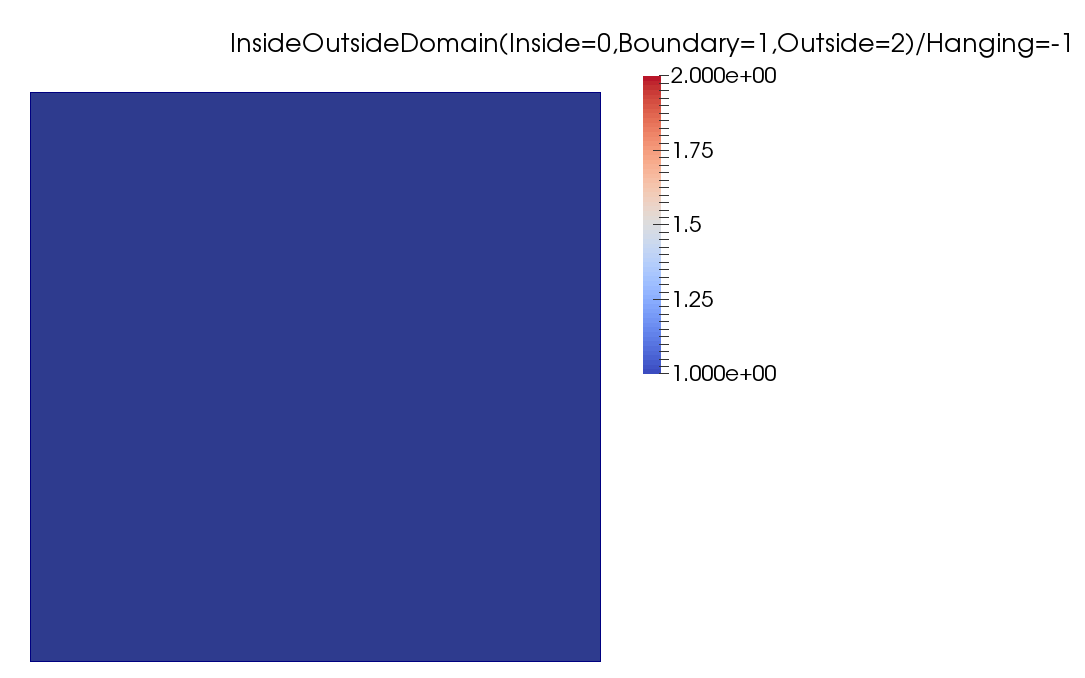
\includegraphics[width=0.8\textwidth]{10_quickstart/screenshot00.png}
\end{center}

\noindent
Congratulations: We have created the simplest adaptive Cartesian grid in 2d that
does exist. A single square!


\section{Some real AMR}

We now set up something slightly more complicated. 
First of all, we switch to a 3d setup rather than 2d. 
For this, open the makefile (\texttt{myproject/makefile}) and alter the
content of the \texttt{DIM} variable.

\begin{code}
# Set Dimension
# -------------
#DIM=-DDim2
DIM=-DDim3
#DIM=-DDim4
\end{code}

\noindent
If you clean your project (\texttt{make -f myproject/makefile clean}) and
rebuild your code, you see that the individual files are translated with the
compile switch 

\begin{code}
g++ ... -DDim3 ....
\end{code}

\noindent
Indeed, this is all that's required for Peano to run a 3d experiment rather than
a 2d setup. 

\begin{remark}
We do support currently up to 10-dimensional setups. If you require higher
dimensions, you might even be able to extend Peano accordingly by changing
solely the file \texttt{peano/utils/Dimensions.h}. But have fun with your memory
requirements exploding.
\end{remark}


Next, we will edit the file \texttt{myproject/mappings/CreateGrid.cpp}. 
Open it with your favourite text editor and search for the operation
\texttt{createBoundaryVertex}. 
Change it into the code below:


\begin{code}
void myproject::mappings::CreateGrid::createBoundaryVertex(
 myproject::Vertex&                          fineGridVertex,
 const tarch::la::Vector<DIMENSIONS,double>& fineGridX,
 const tarch::la::Vector<DIMENSIONS,double>& fineGridH,
 myproject::Vertex * const                   coarseGridVertices,
 const peano::grid::VertexEnumerator&     coarseGridVerticesEnumerator,
 myproject::Cell&                            coarseGridCell,
 const tarch::la::Vector<DIMENSIONS,int>&    fineGridPositionOfVertex
) {
  logTraceInWith6Arguments("createBoundaryVertex(...)", ...); 
    // leave this first line as it is
   
  if (coarseGridVerticesEnumerator.getLevel()<2) {
    fineGridVertex.refine();
  }

  logTraceOutWith1Argument("createBoundaryVertex(...)",fineGridVertex);
}
\end{code}


\noindent
If you compile this code and run the executable, you will (besides lots of
debug output) obtain a way bigger vtk file. 
If you visualise it this time, we observe that the code refines towards the
cube's boundary. 
You may want to play around with magic \texttt{2} in the operation above. 
Or you might want to continue to our final example.

\begin{center}
  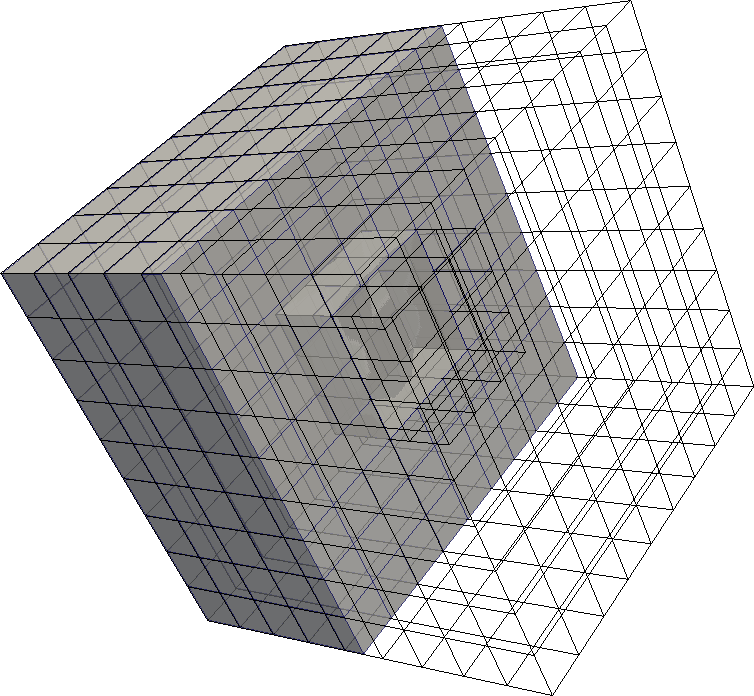
\includegraphics[width=0.55\textwidth]{10_quickstart/cube.png}
\end{center}


\section{A tree within the spacetree}

In the final example we create a slightly more interesting setup. 
We solely edit the operation \texttt{createInnerVertex} within the  
file \texttt{myproject/mappings/CreateGrid.cpp}, recompile it and 
have a look at the result.
When you study source code, please note the similarity to Matlab when we work
with vectors in Peano; as well as that the indices start with 0.
If your want to get rid of all the debug statements and are sick of long 
waiting times, remove the \texttt{-DDebug} statement in the line  
\texttt{PROJECT\_CFLAGS = -DDebug -DAsserts}
within the makefile.
There are more elegant ways to filter out log statements that we will discuss
later.


\begin{code}

void myproject::mappings::CreateGrid::createInnerVertex(
 myproject::Vertex&                          fineGridVertex,
 const tarch::la::Vector<DIMENSIONS,double>& fineGridX,
 const tarch::la::Vector<DIMENSIONS,double>& fineGridH,
 myproject::Vertex * const                   coarseGridVertices,
 const peano::grid::VertexEnumerator&      coarseGridVerticesEnumerator,
 myproject::Cell&                            coarseGridCell,
 const tarch::la::Vector<DIMENSIONS,int>&    fineGridPositionOfVertex 
) {
 logTraceInWith6Arguments("createInnerVertex(...)",fineGridVertex,...);
  
 if (
   fineGridVertex.getRefinementControl()==Vertex::Records::Unrefined 
   &&
   coarseGridVerticesEnumerator.getLevel()<4
 ) {
   bool trunk = (fineGridX(0)-0.5)*(fineGridX(0)-0.5)
              + (fineGridX(2)-0.5)*(fineGridX(2)-0.5)<0.008;
   bool treeTop = (fineGridX(0)-0.5)*(fineGridX(0)-0.5)
                + (fineGridX(1)-0.7)*(fineGridX(1)-0.7)
                + (fineGridX(2)-0.5)*(fineGridX(2)-0.5)<0.3*0.3;
   if (trunk | treeTop) {
     fineGridVertex.refine();
   }
 }

 logTraceOutWith1Argument("createInnerVertex(...)",fineGridVertex);
}
\end{code}

So here's what I get. Feel free to create better pics:

\begin{center}
  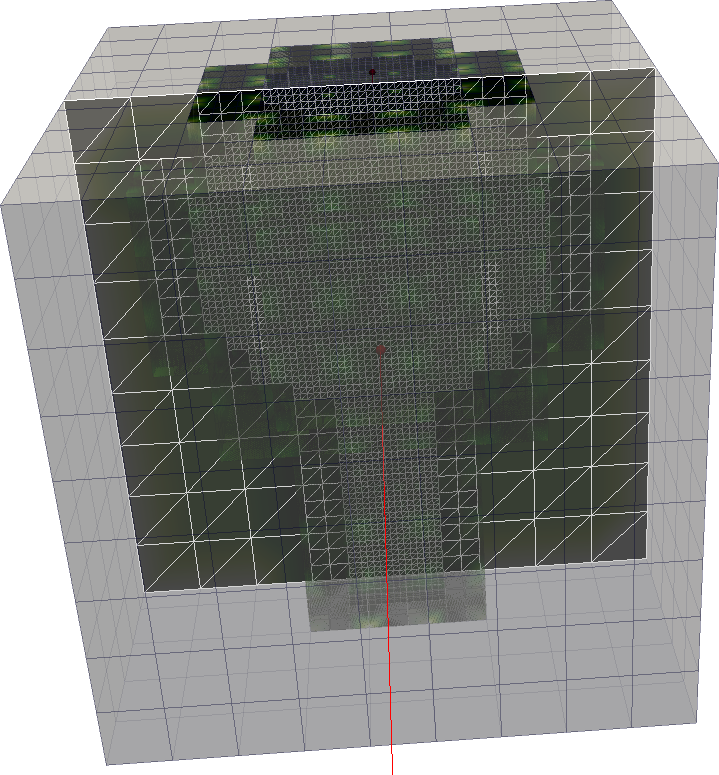
\includegraphics[width=0.55\textwidth]{10_quickstart/tree.png}
\end{center}


 \chapter{Basic Programming Course}
\label{chapter:basics-explained}


\chapterDescription
  {
    15 minutes for the programming but perhaps around 30 minutes for the
    visualisation.
  }
  {
    Chapter \ref{chapter:quickstart}.
  }


In this section, we study a 2d example.
Please adopt your makefile accordingly.
Furthermore, we use the files \texttt{VTKMultilevelGridVisualiserHeader} and
\texttt{...Implementation} as well as
\texttt{VTK2dTreeVisualiser...}.
If you have downloaded the whole Peano repository, these files can be found in
\texttt{pdt/usrtemplates}.
If not, you have to download them manually from the webpage.
Please set up an empty project as discussed in Chapter
\ref{chapter:quickstart} and implement one operation as follows (all other
operations can remain empty/only filled with log statements):


\begin{code}
void myproject::mappings::CreateGrid::touchVertexLastTime(
      myproject::Vertex&               fineGridVertex,
      const tarch::la::Vector<DIMENSIONS,double>&                          fineGridX,
      const tarch::la::Vector<DIMENSIONS,double>&                          fineGridH,
      myproject::Vertex * const        coarseGridVertices,
      const peano::grid::VertexEnumerator&                coarseGridVerticesEnumerator,
      myproject::Cell&                 coarseGridCell,
      const tarch::la::Vector<DIMENSIONS,int>&                             fineGridPositionOfVertex
) {
  logTraceInWith6Arguments( "touchVertexFirstTime(...)", fineGridVertex, fineGridX, ...

  if (
    coarseGridVerticesEnumerator.getLevel()<5
    &&
    tarch::la::equals( fineGridX, 0.0 )
    &&
    fineGridVertex.getRefinementControl()==Vertex::Records::Unrefined
  ) {
    fineGridVertex.refine();
  }

  logTraceOutWith1Argument( "touchVertexFirstTime(...)", fineGridVertex );
}

\end{code}


\noindent
This source fragment requires some additional explanation. 
We neglect the enumerator stuff for the time being.
That will become clear later throughout the present chapter.
The refinement control check says `well, refine, but do it only on unrefined
vertices'.
It's just a matter of good style, not to call \texttt{refine} on a refined
vertex.
The middle line uses a function from the tarch's linear algebra namespace. 
It takes the \texttt{fineGridX} vector (the position of the vertex in space) and
checks whether all entries equal zero.
As we are working with floating point numbers, it is not a bit-wise check. 
Instead, it uses an interval of machine precision around zero.
You may want to change this notion of machine precision in Peano (file
\texttt{Scalar} within the \texttt{tarch::la} namespace). 
In general, it would be a good idea to study the content of the \texttt{la}
component soon---there's lots of useful stuff in there to work with
tiny, dense vectors\footnote{Peano someday should perhaps be rewritten to use
boost linear algebra or some fancy template library. Feel free to do so. Right
at the moment, it is all plain hand-craftet routines.}.

\begin{remark}
  Peano realises a {\bf vertex-based}, {\bf logical-or} refinement: You can
  invoke \texttt{refine} on any unrefined vertex. Peano then refines all cells
  around a vertex in the present or next traversal (it basically tries to do it
  asap, but sometimes data consistency constraints require it to postpone the
  actual refinement by one iteration). The other way round, you may read it as
  follows: A cell is refined if the refinement flag is set for any adjacent
  vertex.
\end{remark}


Whenever you use Peano, you have to do three things:
\begin{enumerate}
  \item Decide which algorithmic phases do exist and in which order they are
  called. Examples for algorithmic phases could be: set up grid, initialise all
  variables, refine regions of interest, perform an iterative solve step, plot
  some data, compute metrics on the solution, \ldots
  \item Model the data, i.e.~decide which data is assigned to the vertices and
  cells of the grid.
  \item Implement the different actions on this data model that are used by the
  algorithmic phases.
\end{enumerate}

This scheme lacks the bullet point `run through the grid'. 
Indeed, Peano applications do never run themselves through the spacetree.
They specify which set of operations is to be called throughout a run through
the grid, i.e.~they say what is done on which data.
Afterward, they invoke the iteration and leave it to Peano to run through the
grid and invoke these operations in the right order on the right ranks using all
the cores you have on your machine\footnote{This statements requires
explanation, and indeed it is not {\em that} straightforward. But the idea is
phrases correctly: the application codes specifies what is to be done and then
outsources the scheduling and the responsibility to use a multicore machine to
Peano.}.
This scheme realises something people call `The Hollywood Principle': Don't
call us, we call you!


\begin{remark}
  The {\bf inversion of control} is the fundamental difference of Peano to other
  spacetree-based codes offered as a library. 
  And typically it is the property many users first struggle with.
  Often, people claim `I have to run through the grid this and that way'. 
  Often, they are wrong.
  It can become quite comfortable to leave it to someone else to decide how 
  grid traversals are realised.
  And it allows the grid traversal in turn to optimise the code under the hook
  without an application developer to bother.
\end{remark}


\section{On the power of loosing control}

The algorithmic phases, i.e.~what can be done on a grid, are specified in the
specification file.
Open your project's file. 
There are two different parts of the document that are of interest to us:
An {\em event mapping} is an algorithmic step that you have to implement
yourself.
In this chapter's example, we want to do two things: create a grid and count all
the vertices. 
Furthermore, we want to plot our grid, but let's keep in mind that Peano has
some predefined actions as well.
So we augment our mapping set as follows:

\begin{code}
// Creates the grid
event-mapping:
  name: CreateGrid

// Counts all the vertices within the grid
event-mapping:
  name: CountVertices
\end{code}

\noindent
Event mappings cannot be used directly.
Instead, we have to specify adapters. 
Adapters take the tree traversal and invoke for each grid part a set of events. 
As we distinguish adapters which basically just glue together (multiple) events
from the events themselves, we will be able to do the following later:
we write a fancy visualisation routine, a routine that adopts the grid to a new
data set and some compute routines.
As we have done this in three different event sets, we can then combine these
events in various ways: compute something and at the same time plot, compute
only, plot and afterward adopt the grid, and so forth.
For the time being, we use the following adapters:

\begin{code}
adapter:
  name: CreateGrid
  merge-with-user-defined-mapping: CreateGrid

adapter:
  name: CountVertices
  merge-with-user-defined-mapping: CountVertices

adapter:
  name: CreateGridAndPlot
  merge-with-user-defined-mapping: CreateGrid
  merge-with-predefined-mapping: VTKGridVisualiser(finegrid)
  merge-with-predefined-mapping: VTKMultilevelGridVisualiser(grid)

adapter:
  name: CountVerticesAndPlot
  merge-with-user-defined-mapping: CountVertices
  merge-with-predefined-mapping: VTKMultilevelGridVisualiser(grid)

adapter:
  name: Plot
  merge-with-predefined-mapping: VTKGridVisualiser(finalgrid)
\end{code}

The first two adapters are trivial: 
They basically delegate to one event set. 
The next two take one event set each and invoke it. 
Furthermore, they also use a predefined event set. 
They will call \texttt{CreateGrid} or \texttt{CountVertices}, respectively, and
at the same time plot.
If you create all code with 

\begin{code}
java -jar <mypath>/pdt.jar --generate-gluecode
myproject/project.peano-specification myproject <mypath>/usrtemplates
\end{code}

\noindent
it is the directory \texttt{usrtemplate} where the PDT searches for the
predefined event sets.
The last adapter by the way is a trivil one, too: It invokes only one of the
events that ship with Peano.


Next, please create all glue code and have a quick look into the file
\texttt{runners/Runner.cpp}.
This file is the starting point of Peano.
The C++ main routine does some setup steps and then creates an instance of the
Runner (see the source code yourself if you don't believe).
It then invokes \texttt{run()} which in turn continues to \texttt{runAsMaster}
or \texttt{runAsWorker()}.
The latter will play a role once we use MPI.
For the time being, let's focus on the master's routine.
Here, we see the following:

\begin{code}
int myproject::runners::Runner::runAsMaster(myproject::repositories::Repository& repository) {
  peano::utils::UserInterface userInterface;
  userInterface.writeHeader();

  // @todo Insert your code here
  
  // Start of dummy implementation
  
  repository.switchToCreateGrid(); repository.iterate();
  repository.switchToCountVertices(); repository.iterate();
  repository.switchToCreateGridAndPlot(); repository.iterate();
  repository.switchToCountVerticesAndPlot(); repository.iterate();
  repository.switchToPlot(); repository.iterate();

 
 
  repository.logIterationStatistics();
  repository.terminate();
  // End of dummy implementation

  return 0;
}
\end{code}

The PDT cannot know what exactly we do, so it basically runs all the adapters we
have specified.
This is the place where we implement our overall algorithm, i.e.~the big
picture.
Lets change it as follows:

\begin{code}
  peano::utils::UserInterface userInterface;
  userInterface.writeHeader();

  repository.switchToCreateGridAndPlot();
  for (int i=0; i<10; i++) repository.iterate();
  repository.switchToCountVertices(); repository.iterate();

  repository.logIterationStatistics();
  repository.terminate();

  return 0;
\end{code}

\noindent
This algorithm says that we want to create a grid and at the same time plot it.
We want to do this ten times in a row.
Afterward, we switch to our vertex counting and want to run through the grid
once more. 
This time, nothing shall be plotted.
We just want to know how many vertices there are.


We really do not care about how the code runs through the grid.
We also do not really care how all vertices, cells, whatever are processed.
We say what is done in which order from a bird eye's perspective.
If you compile the code and run it now, you should end up with a sequence of vtk
files. 
You might want to make a video (take the files that are called
\texttt{finegrid-}something).
Below are some screenshots:


\begin{center}
  
\includegraphics[width=0.3\textwidth]{11_basics/grid00.png}
  
\includegraphics[width=0.3\textwidth]{11_basics/grid01.png}
  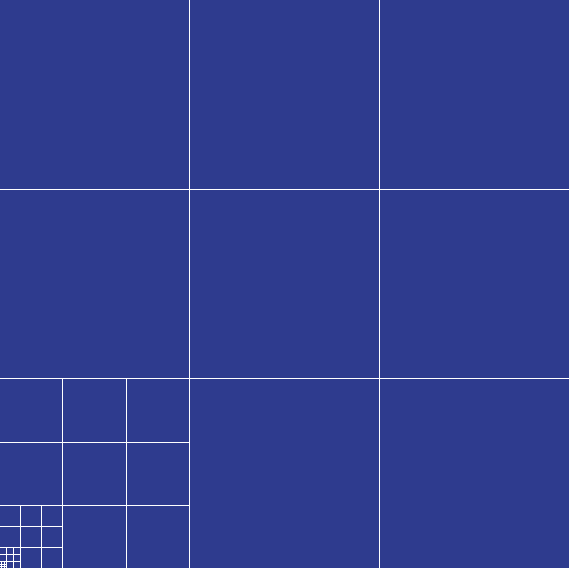
\includegraphics[width=0.3\textwidth]{11_basics/grid02.png}
\end{center}


\section{What happens}


\begin{center}
  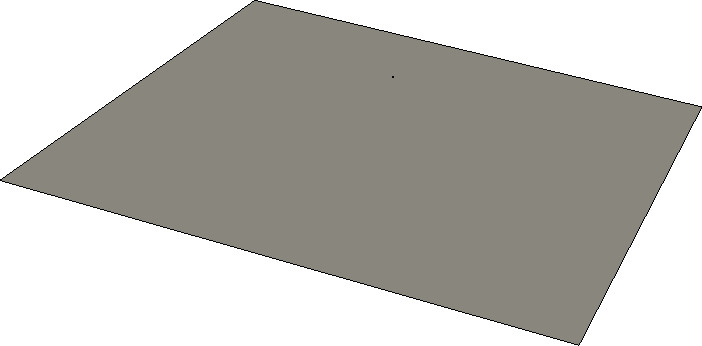
\includegraphics[width=0.45\textwidth]{11_basics/construction00.png}
  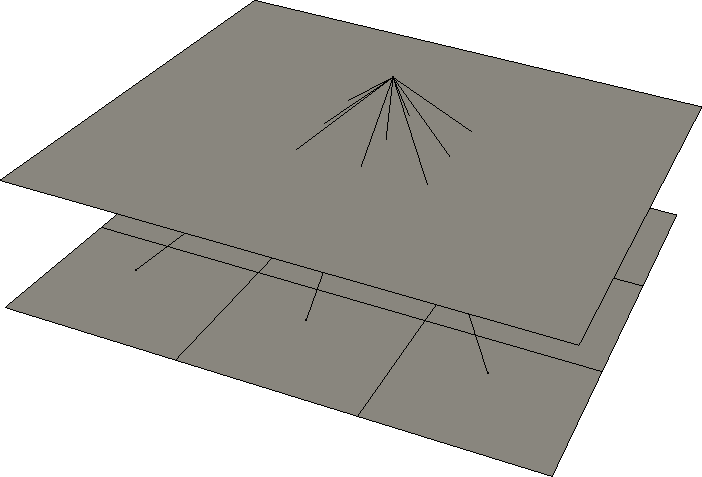
\includegraphics[width=0.45\textwidth]{11_basics/construction01.png}
  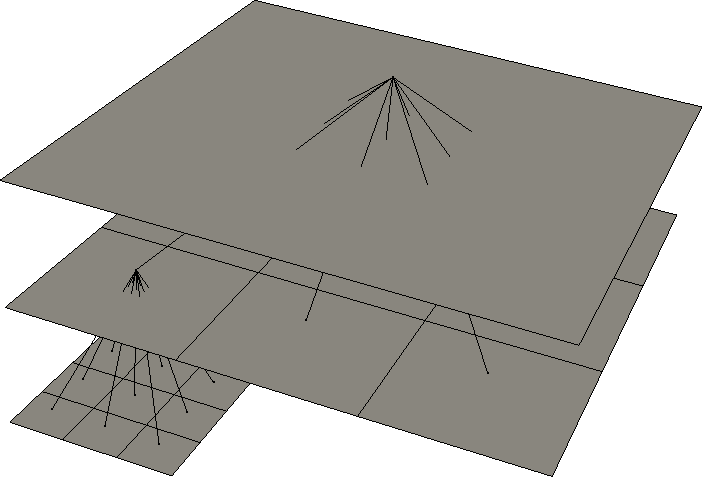
\includegraphics[width=0.45\textwidth]{11_basics/construction02.png}
  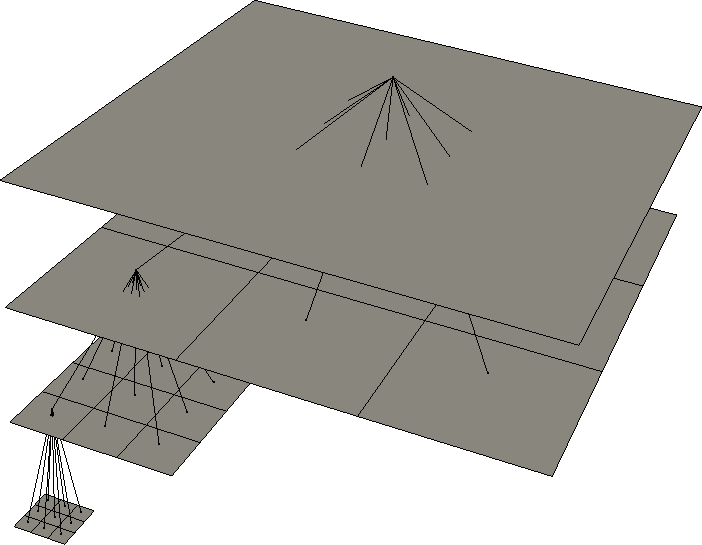
\includegraphics[width=0.45\textwidth]{11_basics/construction03.png}
\end{center}

% UserInterface interpretieren
% Welche events sind da
% was passiert
% Log lesen
% 
% 



\section{Data model}
Prior to a discussion of Peano's data model, it might make sense to load all the
files \texttt{grid-level-?-0.vtk} into your favourite visualisation software.
Dilate them according to their level encoded in the name.
In Paraview, you have to select each file, apply
Filters/Alphabetical/Transform, and dilate each file by -0.2 along the z-axis
per level.
You might end up with something alike:



\begin{center}
  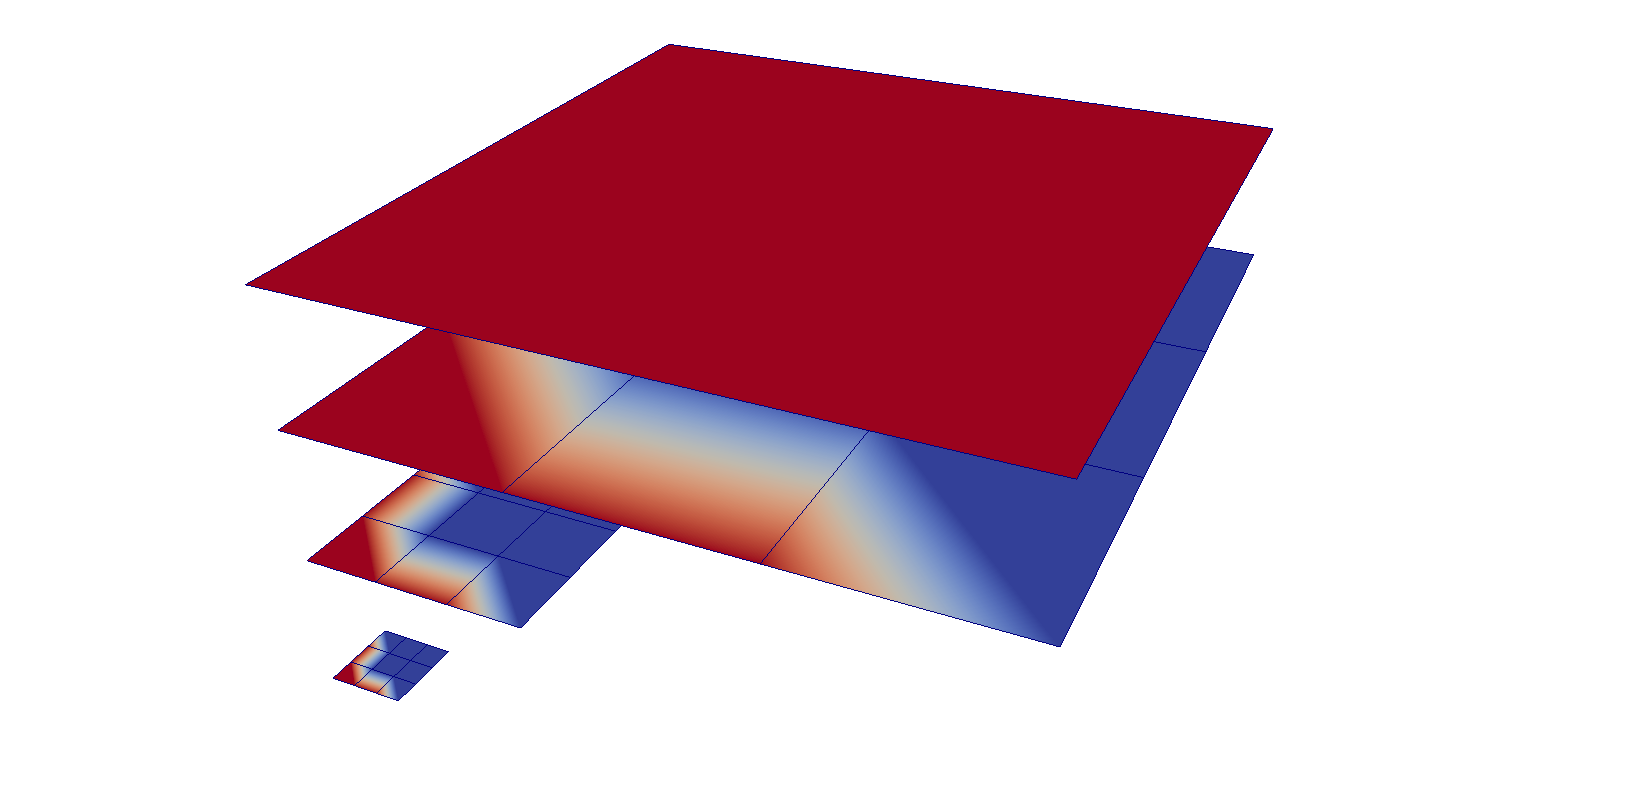
\includegraphics[width=0.8\textwidth]{11_basics/tree00.png}
\end{center}

\noindent
Again, feel free to create a video that shows how additional levels are added in
each step.
There's a more elegant way to end up with a similar picture. 
I once created a graph visualiser that is today also available as predefined
mapping. Just modify your adapters as follows:

\begin{code}
adapter:
  name: CreateGridAndPlot
  merge-with-user-defined-mapping: CreateGrid
  merge-with-predefined-mapping: VTK2dTreeVisualiser(tree,getLevel)
\end{code}

\noindent
This time, creating a video should be straightforward.
\begin{center}
  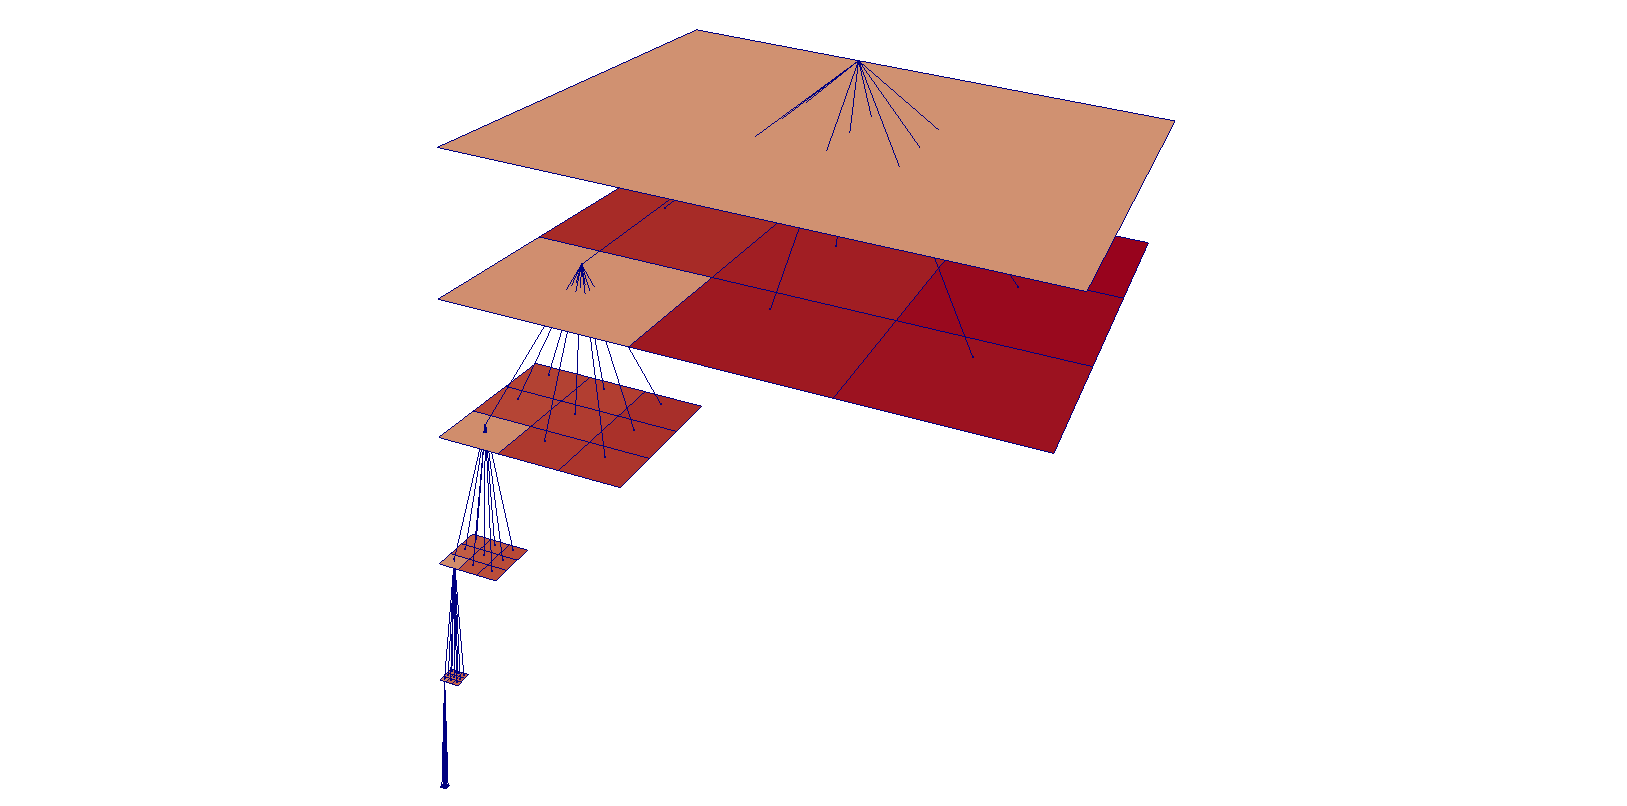
\includegraphics[width=0.8\textwidth]{11_basics/tree01.png}
\end{center}

% Data Model
% Visualisierung von Einbettung
% Wo liegen welche Daten
% 
% Remark: How to realise degrees of freedom associated to faces or edges
% 


\section{Counting vertices}
% We could use the repository's operations
% Do it yourself and then compare
% Finale: Vertices zaehlen
% Den Wert von einem double umsetzen




% \begin{itemize}
%   \item Nochmal eine Beschreibung?
%   \item Welche Paper (auflisten bzw.~referenzieren)
%   \item Academic CV
%   \item Didactic education and awards
%   \item Lecture evaluations
%   \item Involved projects
%   \item Supervised students
%   \item Alle Publikationen
%   \item Weitere Planung
% \end{itemize}

\end{document}
